\chapter{Benchmarks}\label{chap:benchmarks}

We created the \tiles library because our port of the \react into the Dart language was slow. 
Natural question arises. Is the \tiles library faster then the \react port into the dart?

\textit{
	We don't compare the \react library with the \tiles library, we compare the port of it into the dart. 
	The main problem in the port performance was the communication between the JavaScript \react library and the implementation created in the Dart language.
}

We measured the time of several distinct scenarios:
\begin{description}
	\item[The mass vs. the structure] \hfill \\
		We will measure the time, needed to render the mass of components in the same level, 
		and to render the complicated structure with lot of branching.
	\item[Creating of the virutal DOM vs. rendering into the real one] \hfill \\
		We measured the time of the construction of the virtual DOM and the render it into the real one. 
		The measurement is compared between the port and the \tiles library.
	\item[Clean vs. dirty updates] \hfill \\
		The last measurement is the comparison of the duration of the updates. 
		We distinguish two types of updates, clean without any change in the virtual DOM and dirty which changes the virtual DOM.
\end{description}

\section{Benchmarking system}\label{sec:benchmarks-system}

We created the benchmarking system, which compares the \react port with the \tiles library.
The system contain the wrapper class, which enable implementation of a common component for both solutions.
We also implements the benchmark component, used for creation of different structures by passing corresponding props.

The benchmark component get props with two important parameters: 
\begin{description}
	\item[levels] is list of numbers, where each number tells, how many children will have the component on each level,
	\item[level] is the level of the current component.
\end{description}

The component render \texttt{levels[level]} children, all with the level bigger by 1.
If the component is at the last level, it renders corresponding number of \texttt{div}s instead of custom components.

By the benchmark component, we are able to test different type of a structure (flat, deep, etc.).

We implemented a runner which obtain run attributes from the hash of the currently opened site. 
The runner enable to run and collect information about benchmarked tasks by running the \textit{content\textunderscore shell} from a command line.

To collect all informations, we created a shell script, which runs the runner with appropriate parameters and output benchmarked times in CSV format.

\section{Mass versus structure}\label{sec:benchmarks-mass-vs-structure}

	In this benchmark, we compared the render time of the \react port and the \tiles library.
	\begin{figure}[h]
	\centering  
		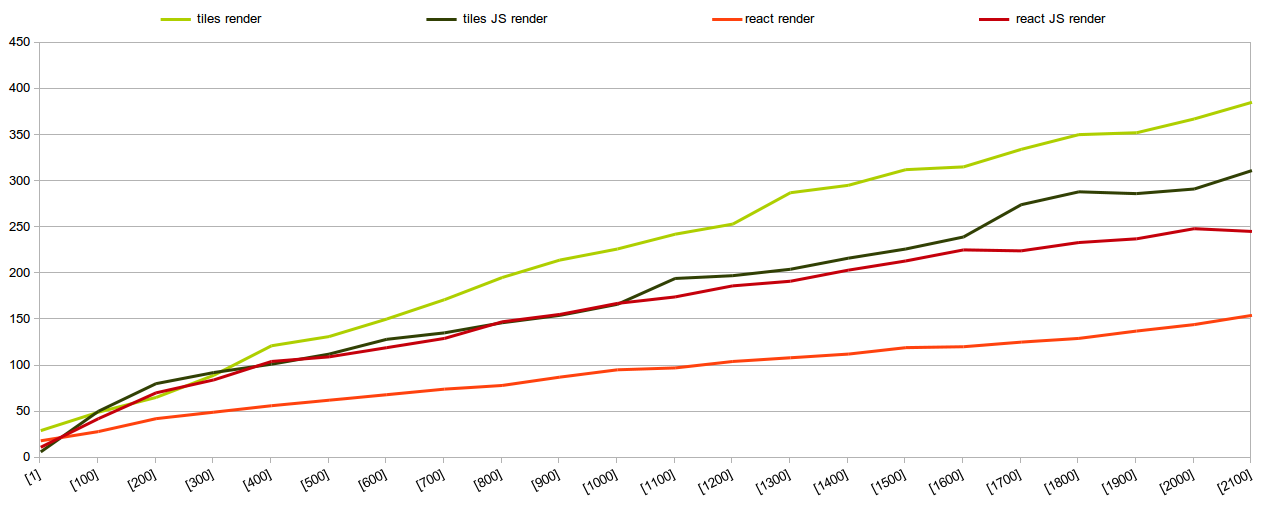
\includegraphics[scale=0.5]{images/benchmarks/m_render.png}
		\caption{Render of simple structure with one custom component and mass of div components}
		\label{img:benchmarks-mass-render}
	\end{figure}

	\begin{figure}[h]
	\centering  
		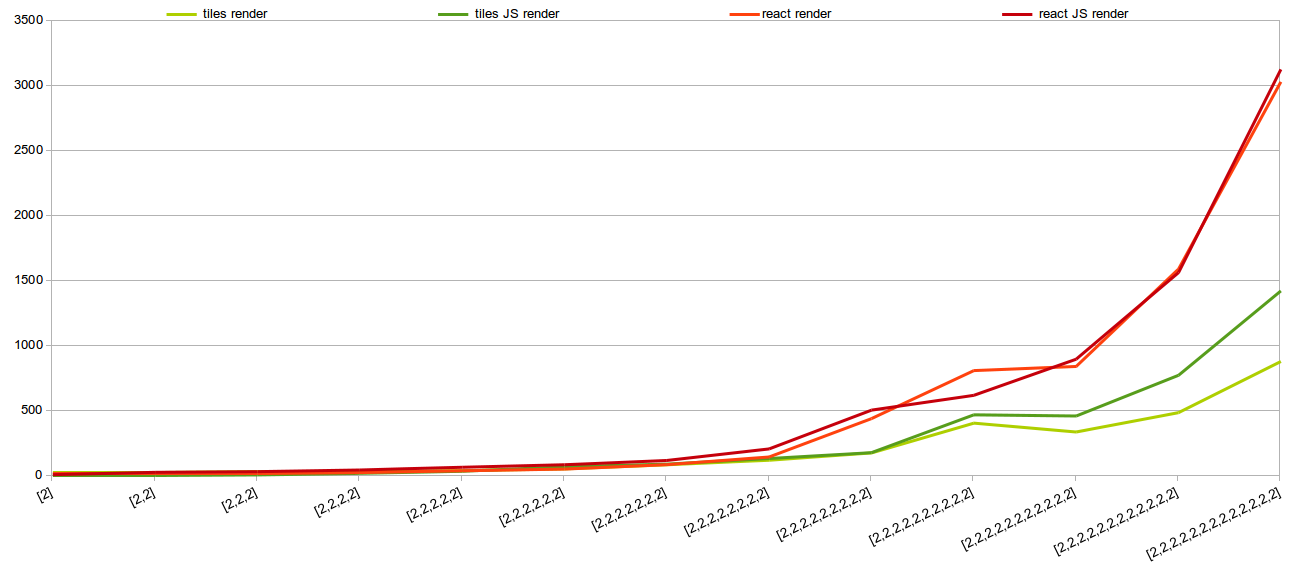
\includegraphics[scale=0.5]{images/benchmarks/s_render.png}
		\caption{Render of structure of custom components}
		\label{img:benchmarks-structure-render}
	\end{figure}

	\begin{figure}[h]
	\centering  
		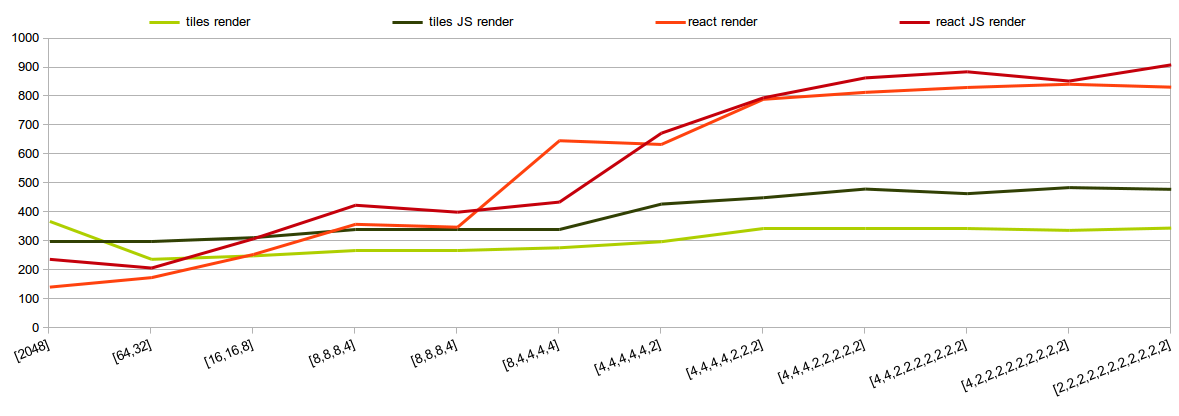
\includegraphics[scale=0.55]{images/benchmarks/mvs_render.png}
		\caption{Comparison of the render of the same number of leafs in the simple, and complicated structure}
		\label{img:benchmarks-mass-vs-structure-render}
	\end{figure}

\section{Clean versus dirty update}\label{sec:benchmarks-clean-vs-dirty-update}

	\begin{figure}[h]
	\centering  
		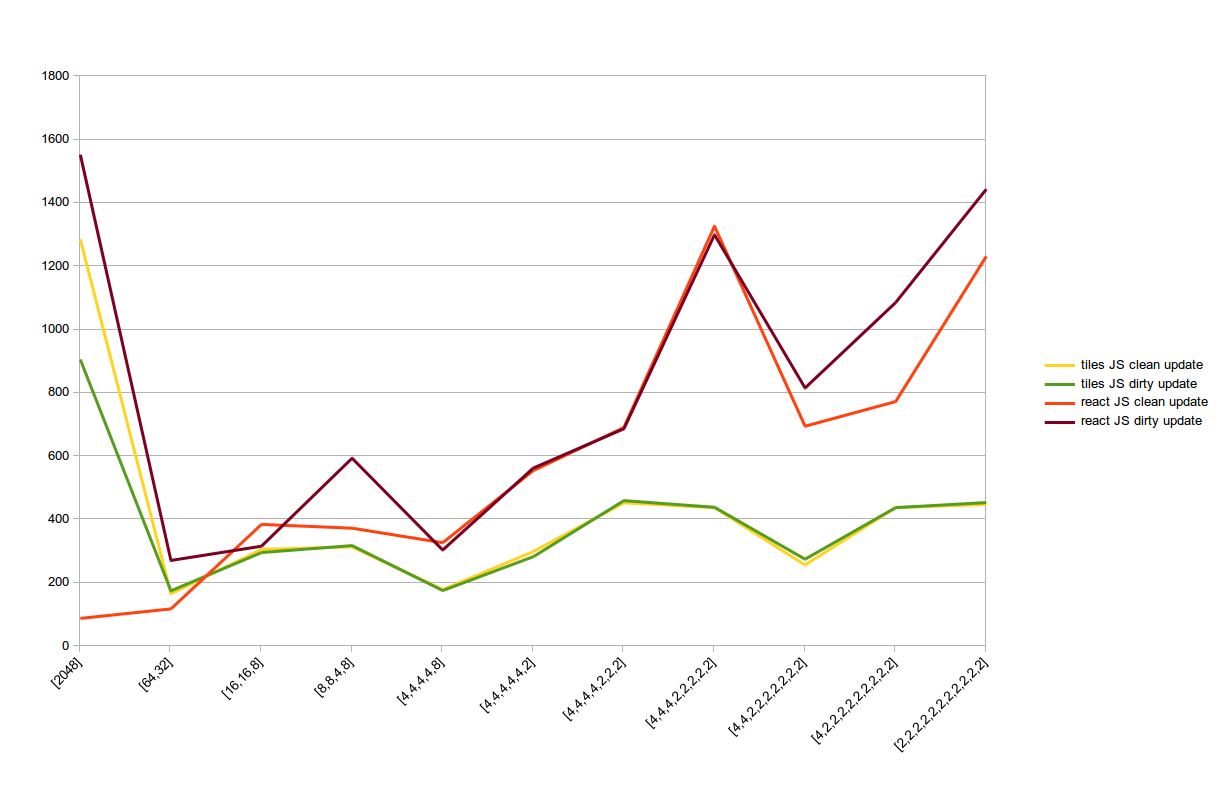
\includegraphics[scale=0.5]{images/benchmarks/mvs_dirty_vs_clean_update.png}
		\caption{Comparison of the clean and dirty update in mass and structure}
		\label{img:benchmarks-mass-vs-structure-dirty-vs-clean-update}
	\end{figure}


\section{Virtual versus real DOM}\label{sec:benchmarks-clean-vs-dirty-update}

	\begin{figure}[h]
	\centering  
		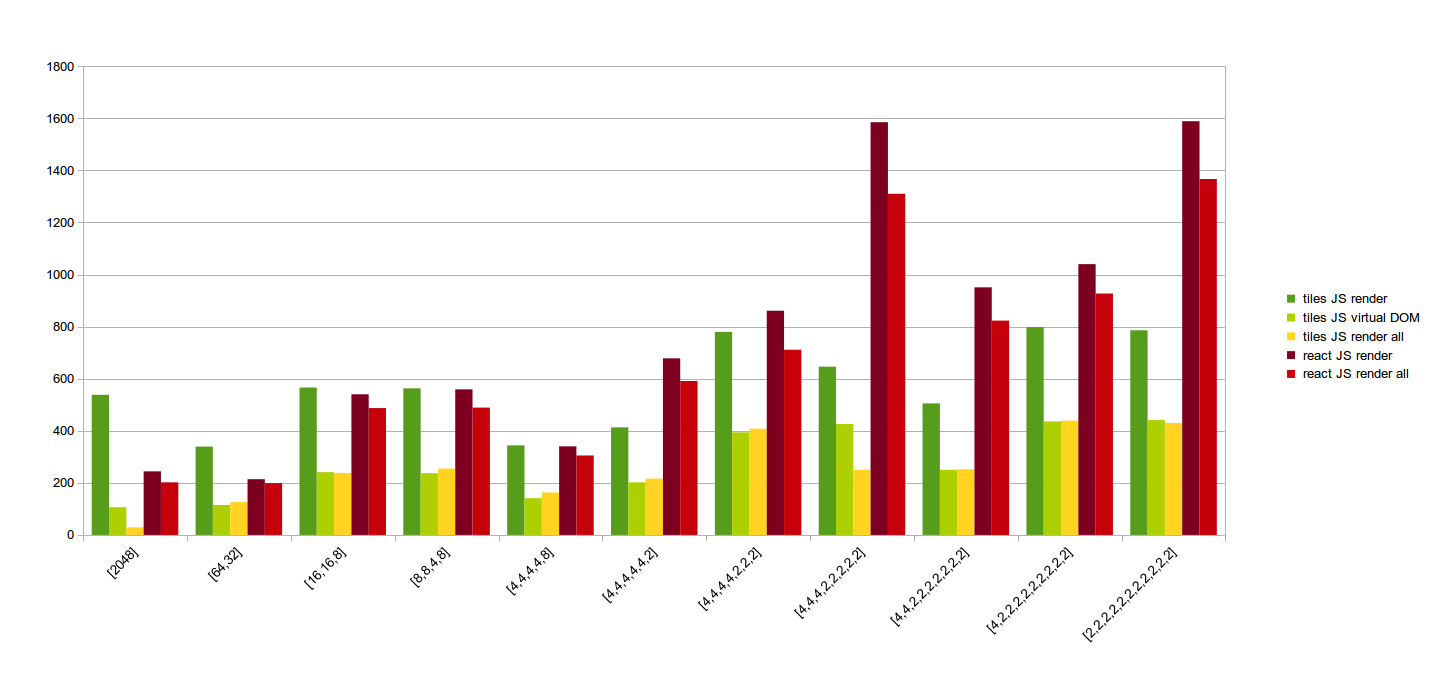
\includegraphics[scale=0.5]{images/benchmarks/mvs_render_vs_virtual_.png}
		\caption{Comparison of the creation of the virtual DOM and rendering into the real DOM in mass and structure}
		\label{img:benchmarks-mass-vs-structure-virtual-vs-real}
	\end{figure}

	\begin{figure}[h]
	\centering  
		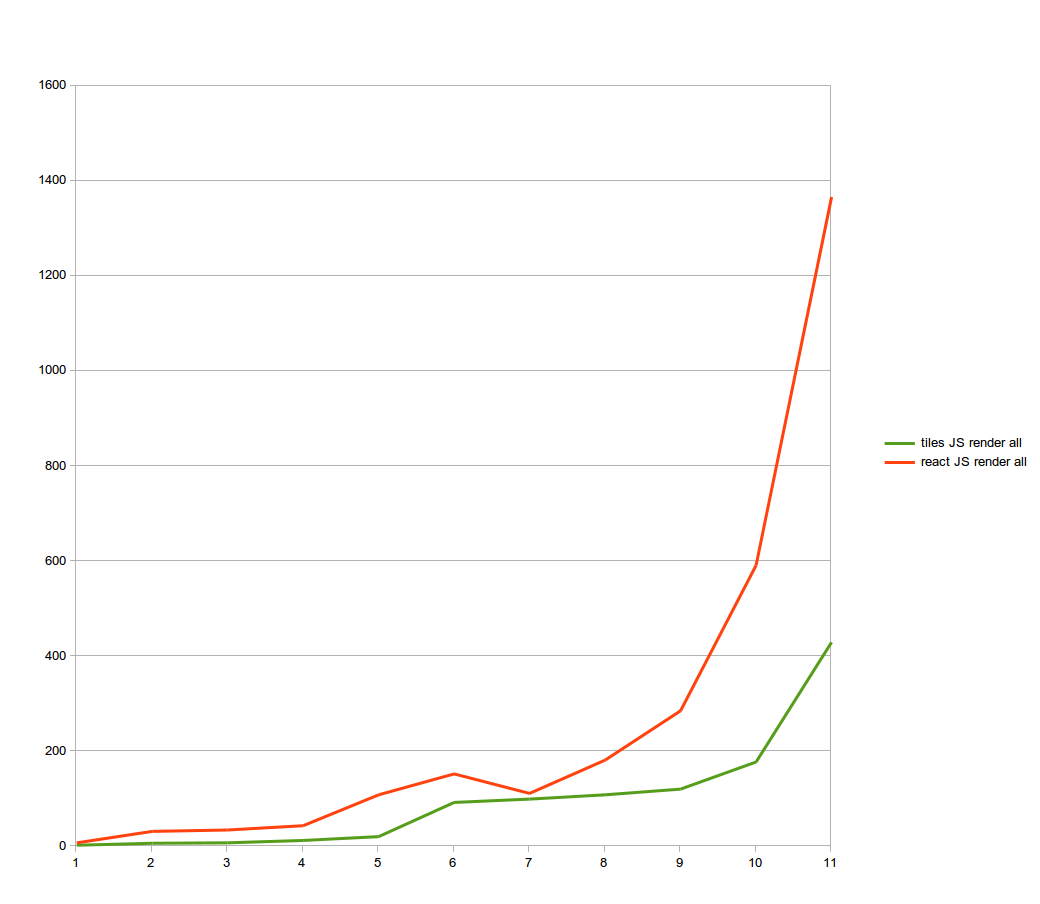
\includegraphics[scale=0.5]{images/benchmarks/s_render_all.png}
		\caption{Comparison of the creation of the virtual DOM and rendering into the real DOM in the structure}
		\label{img:benchmarks-structure-virtual-vs-real}
	\end{figure}

